\chapter[\textit{Testing} Basado en Modelos]{Fundamentos del \textit{testing} basado en modelos}
\label{cap:fundamentos}

En este capítulo introduciremos algunos conceptos básicos con los que trabajaremos a lo largo de esta tesina. Presentaremos el \textit{testing} basado en modelos y veremos mediante un ejemplo como derivar clases y casos de prueba a partir de una especificación Z. Además, presentaremos el funcionamiento de Fastest, la herramienta utilizada para generar clases y casos de prueba de manera automática, en la que basaremos todo el desarrollo a realizar como parte de este trabajo. Finalmente estudiaremos el importante rol que cumplirán las designaciones nuestro sistema de NLG, fundamental para la generación de textos independientes del dominio de aplicación.

\section{\textit{Testing} basado en modelos}

La hipótesis fundamental detrás del \textit{testing} basado en modelos (MBT) es que un programa es correcto si verifica su especificación, entonces, la especificación resulta una excelente fuente para obtener casos de prueba. Las técnicas de MBT utilizan la especificación, en primer instancia, para derivar casos de pruebas abstractos (al nivel del modelo). Estos luego deben ser refinados al nivel del lenguaje de implementación y ejecutados por el programa que supuestamente implementa la especificación. Finalmente la salida del programa será abstraída al nivel de la especificación y la misma será utilizada (nuevamente) para verificar si el caso de prueba ha detectado un error. En el esquema de la figura~\ref{fig:proc_mbt} podemos ver el proceso recién mencionado.

\begin{figure}[H]
\begin{center}
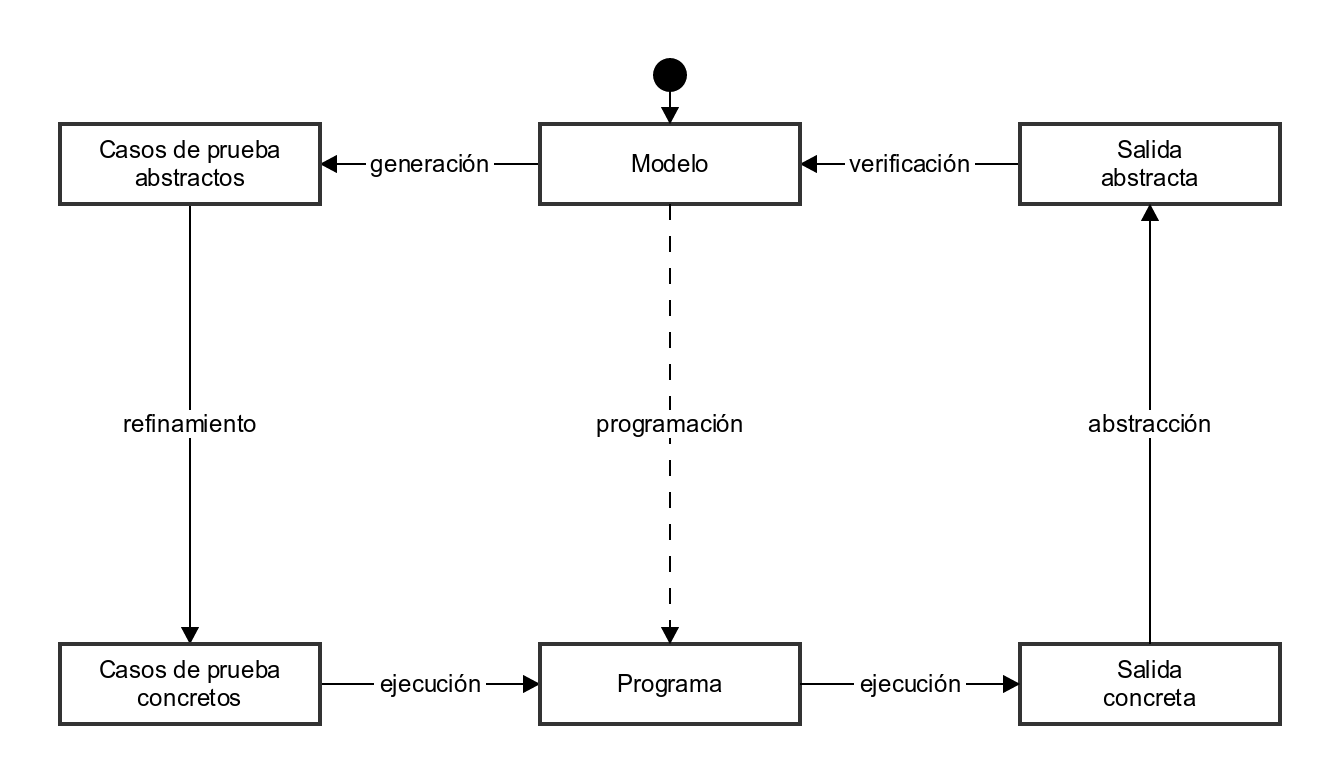
\includegraphics[scale=0.25]{img/proc_mbt.png}
\caption{Proceso de \textit{testing} basado en modelos}
\label{fig:proc_mbt}
\end{center}
\end{figure}


El \textit{Test Template Framework} (TTF) descrito por Stocks y Carrington~\cite{stocks} es un método de MBT que permite efectuar un \textit{testing} muy completo de un sistema del cual se posee una especificación Z~\cite{spivey}, utilizando la misma como entrada y estableciendo cómo generar casos de prueba para testear las distintas operaciones incluidas en el modelo.

A continuación introduciremos brevemente el TTF mediante un ejemplo, asumiendo que el lector se encuentra familiarizado con la notación Z\footnote{Introducción a la notación Z: \url{http://www.fceia.unr.edu.ar/asist/z-a.pdf}}.

\subsection{Ejemplo: \emph{Symbol Table}}
\label{sec:ej-symbolTable}

Una tabla de símbolos es una estructura de datos utilizada por un compilador o intérprete durante el proceso de traducción de un lenguaje de programación donde cada símbolo en el código del programa (variables, constantes, funciones, etc.) se asocia con información como la ubicación, tipo de datos, \textit{scope} de variables, etc. 
En general, en una tabla de símbolos se realizan dos operaciones: inserción y búsqueda; la primera para agregar un símbolo a la tabla y la segunda operación nos permitirá recuperar la información correspondiente a un símbolo ya cargado en la misma.


\bigskip
\noindent
\textbf{Tipos elementales.} Es irrelevante para nuestro modelo especificar en detalle la estructura con la cual representaremos el conjunto de símbolos aceptados por el compilador/interprete, así como la información relativa a los mismos. Para esto, podemos abstraer los conjuntos antes mencionados utilizando los siguientes tipos básicos: 

\begin{zed}
[SYM, VAL] \also
REPORT ::= ok | symbolNotPresent
\end{zed}

El tipo básico \emph{SYM} representará el conjunto de todos los símbolos aceptados por el compilador/interprete, mientras que \emph{VAL} abstraerá el conjunto de toda la información que pudiese estar asociada a un símbolo. Por otro lado, \emph{REPORT} será utilizado para modelar la salida de las operaciones incluidas en la especificación. Una operación podrá ser ejecutada exitosamente o fallar (por ejemplo en caso de realizar una búsqueda de un símbolo que no se encuentre presente en la tabla).
 
\bigskip
\noindent
\textbf{Estado de la tabla.} Es natural pensar que la tabla de símbolos establece una relación funcional entre los símbolos aceptados y la información asociada a cada uno de ellos. Por otro lado, el estado de nuestra tabla está formado únicamente por los símbolos cargados y la información de cada uno. Por lo tanto, podemos modelar el conjuntos de estados de la tabla mediante una única función parcial\footnote{Utilizamos una función parcial ya que no todos los símbolos aceptados por el compilador estarán presentes en la tabla.} de la siguiente manera:

\begin{schema}{ST}
st: SYM \pfun VAL
\end{schema}

\bigskip
\noindent
\textbf{Operaciones.} Como mencionamos anteriormente, dos operaciones se realizarán sobre la tabla de símbolos: inserción y búsqueda.

\bigskip
Comenzaremos por modelar la operación de inserción o actualización. Esta operación modificará el estado de la tabla de símbolos; para esto, será necesario brindarle a la operación el símbolo y la información correspondiente al mismo.

Para actualizar la información de un símbolo en la tabla, simplemente actualizaremos la relación funcional con un par ordenado construido a partir del símbolo y la información dada. 

\begin{schema}{Update}
  \Delta ST \\
  s?: SYM \\
  v?: VAL \\
  rep!: REPORT
  \where
  st' = st \oplus \{s? \mapsto v?\} \\
  rep! = ok
\end{schema}

Por último, deberemos especificar la operación encargada de recuperar la información vinculada a un símbolo. Se trata de una operación relativamente simple que no modifica el estado de la tabla de símbolos. Ésta requerirá de un símbolo a buscar y retornará la información vinculada al mismo. A continuación especificaremos el caso exitoso para esta operación:

\begin{schema}{LookUpOk}
\Xi ST \\
s?: SYM \\
v!: VAL \\
rep!: REPORT
\where
s? \in \dom st \\
v! = st~s? \\
rep! = ok
\end{schema} 

Utilizamos la variable de salida \emph{rep!} para para comunicar el éxito o fracaso de la operación, y la variable \emph{v!} para retornar la información solicitada. 

El esquema \emph{LookUpOk} modela solamente el caso en el que el símbolo a buscar se encuentre cargado en la tabla, pero deberemos contemplar también el caso en que se intente buscar un símbolo que no haya sido cargado en la misma. Modelaremos esta situación con el esquema de error \emph{LookUpE}, presentado a continuación:

\begin{schema}{LookUpE}
\Xi ST \\
s?: SYM \\
rep!: REPORT
\where
s? \notin \dom st \\
rep! = symbolNotPresent
\end{schema}

Finalmente, la operación total (que es la que se debe programar) queda definida de la siguiente manera:

\bigskip
$LookUp == LookUpOk \lor LookUpE$

\subsection{\emph{Test Template Framework}}

La propuesta de Stocks y Carrington~\cite{stocks} es utilizar la especificación Z de una operación como fuente de la cual obtener casos de prueba para testear el programa que supuestamente la implementa. La idea se basa en que la especificación del programa contiene todas las alternativas funcionales que el ingeniero consideró imprescindible describir para que el programador implemente el programa correcto. Por lo tanto, para saber si el programa funciona correctamente es necesario probarlo para cada una de estas alternativas funcionales. 

\subsection{Clases y casos de prueba}

Las alternativas funcionales antes mencionadas pueden expresarse como restricciones sobre las variables de entrada y de estado definidas para la especificación. Estas alternativas pueden ser especificadas mediante esquemas Z a los que llamaremos \emph{clases de prueba}. Por ejemplo:

\begin{zed}
   LookUp_{1}^{DNF} == [st: SYM \pfun VAL; s?: SYM  | s? \in \dom st] \\
\end{zed}

\noindent
define una clase de prueba para el esquema \emph{LookUp}, introducido anteriormente, donde $st$ y $s?$ son variables de estado y de entrada respectivamente, y $s? \in \dom st$ es la restricción sobre las mismas. 

Por otro lado, necesitaremos buscar valores específicos, o constantes, para las variables de una \emph{clase de prueba} (que reduzcan su restricción a verdadero) a fin de luego refinarla y poder ejecutar el caso de prueba en el programa que implemente la especificación. Llamaremos \emph{caso de prueba} a la tupla conformada por los valores correspondientes a cada una de las variables involucradas en la clase de prueba que satisfagan la restricción de ésta. Nos bastará con escoger un único \emph{caso de prueba} para cada clase de prueba generada (observemos que en algunos casos, como por ejemplo para la clase de prueba antes presentada, podríamos encontrar infinitos valores posibles para las variables de la clase de prueba que cumplan con la restricción).

Como mencionamos recientemente, los casos de prueba son tuplas conformadas por constantes correspondientes a cada una de las variables involucradas en las clases de prueba correspondientes. Para los tipos dados por el lenguaje, como por ejemplo $\mathbb Z$, las constantes ya se encuentran definidas en el lenguaje, pero esto no ocurre cuando trabajamos con tipos introducidos por el especificador, como $SYM$ y $VAL$ definidos en el ejemplo que venimos estudiando. En estas circunstancias, será necesario definir constantes para estos tipos de datos a fin de poder luego utilizarlas en nuestros casos de prueba. Continuando con el ejemplo, para $SYM$ y $VAL$ podemos definir:

\begin{axdef}
sym_{1}: SYM \\
val_{1}: VAL
\end{axdef}

Ahora que contamos con estas constantes, estamos en condiciones de definir un caso de prueba para la clase de prueba $LookUp_{1}^{DNF}$ de la siguiente manera:

\begin{figure}[H]
\center
$LookUp_{TC}^{1} == [LookUp_{1}^{DNF}  | st = \{sym_{1} \mapsto val_{1} \} \land s? = sym_{1}]$
\end{figure}

Podemos observar en el caso de prueba presentado que hemos asignamos una constante a cada una de las variables del $VIS$ de forma tal que satisfaga la restricción de la clase de prueba en cuestión.

\subsection{Generación de clases de prueba}
\label{sec:tacticas-testing}

En esta sección introduciremos brevemente, por medio de un ejemplo, el proceso del TTF. Continuaremos trabajando sobre el ejemplo introducido anteriormente e intentaremos generar algunos casos de prueba para testear la operación \emph{LookUp}. En particular nos concentraremos en la generación de clases de prueba, que resultarán de vital interés para nuestro trabajo de NLG.

El primer paso del TTF será definir el espacio de entrada (\emph{IS}, por \emph{Input Space}) para la operación. Este será el conjunto definido por todos los posibles valores de entrada y estado de la misma. Por ejemplo, el \emph{IS} para la operación \emph{LookUp} será:

\begin{zed}
  IS == [st: SYM \pfun VAL; s?: SYM]
\end{zed}

En los casos en los que las operaciones son parciales, no tendrá sentido probar el sistema con casos de prueba para los cuales no está definida la operación, es por esto que, a partir del \emph{IS}, el TTF definirá luego el espacio válido de entrada (\emph{VIS}, por \emph{Valid Input Space}). Este será un subconjunto del anterior, formado por los elementos pertenecientes al \emph{IS} que cumplan con la precondición de la operación en cuestión, es decir:

\begin{zed}
  VIS_{Op} == [IS | pre~Op]
\end{zed}

El \emph{VIS} será un subconjunto del \emph{IS} para los cuales tiene sentido testear el programa. Para el caso de \emph{LookUp} será:

\begin{zed}
  VIS_{LookUp} == IS
\end{zed}

\noindent
ya que la operación es total. El \emph{IS} y el \emph{VIS} no coincidirían si la operación \emph{LookUp}, por ejemplo, no se hubiera incluido el esquema de error. En ese caso tendríamos:

\begin{zed}
  IS == [st: SYM \pfun VAL; s?: SYM] \\
  VIS_{LookUpOk} == [IS | s? \in \dom st]
\end{zed}

Luego de determinar el \emph{VIS}, el TTF propone dividir el mismo, de modo tal que cada una de estas particiones represente una alternativa funcional distinta de la operación a testear. Estas particiones serán las \emph{clases de prueba}, introducidas anteriormente. Para dividir el $VIS$ a fin de dar con éstas, será necesario aplicar alguna estrategia o \emph{táctica de testing} que establezca la forma en la cual puede ser particionado el $VIS$. Luego, será posible aplicar nuevas tácticas sobre estas particiones generadas a fin de dividir nuevamente las mismas, obteniendo como resultado nuevas clases de prueba; este proceso se podrá repetir hasta que el ingeniero de \textit{testing} considere que todas las alternativas funcionales importantes de la operación están representadas (cada una de estas alternativas corresponderá a una única clase de prueba). El último paso del proceso será la selección de al menos un \emph{caso de prueba} para cada clase de prueba, que, como vimos anteriormente, consistirá en buscar valores para las variables de la misma que reduzcan su restricción a verdadero. 

A continuación, mostraremos la aplicación de algunas tácticas de \textit{testing} sobre la operación \emph{LookUp}. En primer lugar aplicaremos Forma Normal Disyuntiva (DNF del inglés \emph{``Disjunctive Normal Form''}) y luego aplicaremos la táctica de Partición Estándar (SP del inglés \emph{``Standard Partition''}) a la expresión: ``$s? \in \dom st$''.

\bigskip
\noindent
\textbf{Forma Normal Disyuntiva.} Suele ser la primer táctica que se aplica. Esta expresará la operación como una disyunción de esquemas en los cuales únicamente habrá conjunciones de literales o de negaciones de literales y luego dividirá el \emph{VIS} con las pre-condiciones de cada esquema. 

Continuando con el ejemplo, \emph{LookUp} ya es una disyunción y cada uno de los esquemas que la forman se encuentra en DNF. Por lo tanto, solo deberemos dividir el \emph{VIS} con la precondición de cada uno de ellos, de la siguiente forma:

\begin{zed}
  LookUp_{1}^{DNF} == [VIS_{LookUp} | s? \in \dom st] \\
  LookUp_{2}^{DNF} == [VIS_{LookUp} | s? \notin \dom st]
\end{zed}

De esta forma obtenemos una partición del \emph{VIS}\footnote{Esto no se cumple en todos los casos, podrían ``solaparse'' las particiones obtenidas, pero de cualquier forma lograríamos un cubrimiento funcional básico.}. Además, observemos que si tomamos un caso de prueba para cada una de las clases obtenidas estaríamos probando el sistema en las siguientes situaciones:

\begin{enumerate}
\item Intentar buscar un símbolo cargado en la tabla de símbolos.
\item Intentar buscar un símbolo que no fue cargado previamente en la tabla de símbolos.
\end{enumerate}

\bigskip
\noindent
\textbf{Partición Estándar.} Esta táctica trata con los operadores matemáticos de una operación. Una partición estándar es una partición del dominio del operador en conjuntos llamados \emph{sub-dominios}. En la figura~\ref{ej:partition_in} podemos ver una partición estándar para los operadores $\in$ y $\notin$.

\begin{figure}[H]
\begin{framed}
  \begin{tabular}{l l l l}
    1. $A = \{\}$ & 3. $A = \{b\}$ & 5. $A = \{b, c\}$  & 7. $\{b, c\} \subset A, a \notin A$ \\ 
    2. $A = \{a\}$ & 4. $A = \{a, b\}$ & 6. $\{a, b\} \subset A$ &   \\ 
  \end{tabular}
  \end{framed}
  \caption{Partición estándar para a $\protect\in$ A; se asume que $a, b \text{ y } c$ son tres elementos diferentes}
  \label{ej:partition_in}
\end{figure}

Para aplicar esta táctica primero hay que seleccionar un operador de un predicado incluido en el esquema de la operación a testear.

Siguiendo con el ejemplo anterior, aplicaremos la técnica de partición estándar a la clase de prueba $LookUp_{1}^{DNF}$. En primer lugar, deberemos seleccionar una aparición de un operador en el esquema de la operación \emph{LookUp}. 
Nosotros elegiremos el operador $\in$ de la expresión ``$s? \in \dom st$''.


El siguiente paso será reemplazar los parámetros formales que aparecen en la descripción de la partición por las expresiones usadas en la especificación.  En particular, para nuestro ejemplo, deberemos reemplazar los parámetros de las expresiones que aparecen en la figura~\ref{ej:partition_in} con las expresiones ``$s?$'' y ``$\dom st$''. Finalmente, a partir de la clase de prueba sobre la cual se quiere aplicar la táctica, tendremos que generar las nuevas particiones para cada uno de los sub-dominios definidos en la partición estándar. En consecuencia, obtendremos las siguientes clases:


\begin{zed}
  LookUp_{1}^{SP} == [LookUp_{1}^{DNF} | \dom st = \{\}] \\
  LookUp_{2}^{SP} == [LookUp_{1}^{DNF} | \dom st = \{s?\}] \\
  LookUp_{3}^{SP} == [LookUp_{1}^{DNF} | \dom st = \{b\}] \\
  LookUp_{4}^{SP} == [LookUp_{1}^{DNF} | \dom st = \{s?, b\}] \\
  LookUp_{5}^{SP} == [LookUp_{1}^{DNF} | \dom st = \{b, c\}] \\
  LookUp_{6}^{SP} == [LookUp_{1}^{DNF} | \{s?, b\} \subset \dom st] \\
  LookUp_{7}^{SP} == [LookUp_{1}^{DNF} | \{b, c\} \subset \dom st \land s? \notin \dom st] \\
\end{zed}

Luego podríamos continuar aplicando nuevas tácticas y particionando aún más el \emph{VIS}. En este caso se trata de una operación relativamente sencilla y consideramos que todas las alternativas funcionales importantes se encuentran representadas mediante las clases de prueba obtenidas.

\subsection{Fastest}
\label{sec:fastest}

\emph{Fastest}\footnote{\url{http://www.fceia.unr.edu.ar/~mcristia/fastest-1.6.tar.gz}} es una herramienta que implementa la teoría del TTF desarrollada en primer instancia por Maximiliano Cristiá y Pablo Rodriguez Monetti~\cite{fastest1}. El desarrollo de la misma fue impulsado para intentar automatizar, lo máximo posible, el proceso de \textit{testing} funcional basado en especificaciones Z. \emph{Fastest} se encuentra implementado mayormente en lenguaje Java y hace uso de las librerías del \textit{framework} CZT\footnote{\url{http://czt.sourceforge.net/}} (\emph{Community Z Tools}) para contar con utilidades relacionadas al lenguaje de especificación Z. 

A continuación, en la figura \ref{ej:comandos_fastest}, ilustraremos el funcionamiento de \emph{Fastest} mostrando los comandos necesarios para generar las clases de prueba introducidas anteriormente en esta sección.


\begin{figure}[H]
\begin{Verbatim}[frame=single,fontsize=\scriptsize]
Fastest version 1.6, (C) 2013, Maximiliano Cristiá
Loading pruning rewrite rules...
Loading pruning theorems...
Fastest> loadspec symbolTable.tex
Loading specification..
Specification loaded.
Fastest> selop LookUp
Fastest> genalltt 
Generating test tree for 'LookUp' operation.
Fastest> addtactic LookUp_DNF_1 SP \in s? \in \dom st
Fastest> genalltt                                    
Fastest> showsch -tcl -u 2

\begin{schema}{LookUp\_ DNF\_ 1}\\
 st : SYM \pfun VAL \\
 s? : SYM 
\where
 s? \in \dom st
\end{schema}

\begin{schema}{LookUp\_ SP\_ 1}\\
 st : SYM \pfun VAL \\
 s? : SYM 
\where
 s? \in \dom st \\
 \dom st = \{ s? \}
\end{schema}

\begin{schema}{LookUp\_ SP\_ 2}\\
 st : SYM \pfun VAL \\
 s? : SYM 
\where
 s? \in \dom st \\
 \dom st \neq \{ s? \} \\
 s? \in \dom st
\end{schema}

\begin{schema}{LookUp\_ DNF\_ 2}\\
 st : SYM \pfun VAL \\
 s? : SYM 
\where
 s? \notin \dom st
\end{schema}
\end{Verbatim}
\caption{Comandos para generación de clases de prueba en \emph{Fastest}}
\label{ej:comandos_fastest}
\end{figure}

Como se podemos observar en la figura \ref{ej:comandos_fastest}, en primera instancia cargamos la especificación en \emph{Fastest} mediante el comando \texttt{loadspec}. \emph{Fastest} realiza algunas verificaciones sintácticas y de tipos sobre la especificación y en caso de encontrar algún error lo informa por pantalla. El comando \texttt{selop} selecciona un esquema con el cual trabajar (para el ejemplo anterior seleccionamos sólo uno, pero es posible seleccionar más esquemas). Luego, \texttt{genaltt} es utilizado, en este caso, para aplicar la táctica de DNF (\emph{Disjunctive Normal Form}); esta táctica es aplicada por defecto la primera vez que es ejecutado el comando. El comando \texttt{addtactic} añadirá una nueva táctica de partición, pero no ejecutará la misma. Será necesario volver a ejecutar \texttt{genaltt} para realizar la partición en base a la táctica ingresada. Finalmente, mostramos por pantalla todas las clases de prueba generadas por \emph{Fastest} utilizando el comando \texttt{showsch} (el parámetro \texttt{-tcl} fue utilizado para indicar que sólo queremos imprimir clases de prueba, mientras que \texttt{-u} fue utilizado para indicarle a \emph{Fastest} que queremos expandir las definiciones de las mismas).

Observemos que \emph{Fastest} utiliza una notación levemente diferente, pero equivalente, a la introducida en este capítulo para nombrar las clases y casos de prueba. En lo que queda de este trabajo, seguiremos estilo propuesto por \emph{Fastest} cuando hagamos referencia a clases y casos de prueba generados por medio de esta herramienta.

En lo que respecta a la generación de lenguaje natural, \emph{Fastest} fue utilizado en el pasado para testear el software a bordo de un satélite~\cite{satelite} y posteriormente se utilizaron técnicas de generación de lenguaje natural basada en \textit{templates} para traducir los casos de prueba obtenidos \cite{cristia_pluss}. La situación propuesta en el trabajo recién mencionado fue una solución ad-hoc, dependiente del dominio de aplicación y de la cantidad de operaciones.


Como mencionamos anteriormente, uno de los objetivos de este trabajo será el de extender la implementación de \emph{Fastest} para permitir al usuario generar descripciones, independientes del dominio de aplicación y de la cantidad de operaciones de las clases de prueba generadas con la herramienta.
El sistema de NLG a desarrollar en este trabajo será íntegramente implementado en Java e integrado como una extensión de \emph{Fastest} (trabajando para esto con la versión 1.6 de la herramienta). En el capítulo \ref{cap:implementacion} veremos algunos de los detalles más relevantes de esta implementación.

\section{Designaciones}
\label{cap:designaciones}

Un modelo formal, como una especificación Z en este caso, es una abstracción de la realidad. Sin embargo, se realiza una especificación para escribir un programa que finalmente es usado en el mundo real. En consecuencia, existe una relación entre el modelo y la realidad.
Normalmente en estos casos, cuando especificamos un sistema formalmente, es una practica común incluir asociaciones entre elementos de la especificación (operaciones, esquemas de estado, variables, constantes, etc.) y elementos que refieran al dominio de aplicación. Estas asociaciones son llamadas \emph{designaciones}~\cite{jackson}.
Sin esta documentación el modelo sería nada más que una teoría axiomática más sin conexión con la realidad. 

Para documentar las designaciones usaremos la sintaxis propuesta por Jackson~\cite{jackson}:

\begin{figure}[H]
  \centering
  \emph{texto informal} $\approx$ \textbf{término\_formal}
\end{figure}

El símbolo $\approx$ demarca la frontera entre el mundo real (a la izquierda) y el mundo formal o lógico (a la derecha). Del lado derecho estará el término formal a designar, este será un elemento de la especificación, mientras que del otro lado tendremos texto informal en lenguaje natural que permitirá reconocer el fenómeno designado.

Continuando con el ejemplo de la tabla de símbolos (sección ~\ref{sec:ej-symbolTable}), podríamos contar (entre otras) con las siguientes designaciones:

\begin{figure}[H]
  \begin{align*} 
    &\text{Símbolo a buscar} && \approx &&&s? \\
    &\text{Información asociada a $x$} && \approx &&&st~x
  \end{align*}
  \caption{Algunas designaciones para \emph{SymbolTable}}
  \label{fig:ej_designacion}
\end{figure}


Para Jackson, las designaciones sirven en primera instancia cuando se empieza a escribir la especificación para diferenciar un fenómeno en particular y darle un nombre. Luego, le será de utilidad al programador a la hora de leer la especificación. Jackson propone construir un \emph{``puente angosto''} entre la especificación y los elementos del dominio, escribiendo la menor cantidad de designaciones posibles y definiendo otros términos en base a las anteriores.


La función que cumplirán las designaciones en éste trabajo difiere un poco de la propuesta por Jackson. Para nosotros las designaciones resultarán la principal fuente de conocimiento para nuestro sistema de NLG. Y serán fundamentales para que éste pueda generar descripciones independientes del dominio de aplicación.

Veamos, por ejemplo, las siguientes expresiones pertenecientes a dos clases de prueba de dos especificaciones distintas:

\begin{figure}[H]
\begin{enumerate}
\item $\dom st = \{ s? \}$
\item $\dom cajas = \{ num? \}$
\end{enumerate}
\end{figure}

La primera expresión pertenece a una clase de prueba generada para la operación \emph{LookUp}, la segunda es parte de una clase de prueba generada para una operación perteneciente a la especificación de un sistema bancario. Estas expresiones resultan equivalentes (de hecho, hasta podríamos haber usado los mismos nombres de variables para ambas especificaciones); será gracias a las designaciones que podremos otorgarles una descripción en lenguaje natural (acorde al dominio de aplicación de cada especificación) a cada una de estas expresiones. En particular, para estas, las descripciones podrían ser las siguientes:

\begin{figure}[H]
\begin{enumerate}
\item \emph{``El símbolo a buscar es el único cargado en la tabla de símbolos.''}
\item \emph{``El número de caja de ahorro ingresado es el único cargado en el banco.''}
\end{enumerate}
\end{figure}

Los sistemas de generación de lenguaje natural generalmente utilizan un diccionario de palabras o frases, las cuales se utilizan para referirse a fenómenos del dominio. En nuestro caso, el dominio de aplicación dependerá de la especificación en cuestión y de lo que se modele con la misma, por lo tanto, las designaciones resultarán nuestra única fuente de textos dependientes del dominio y es por eso que serán un elemento fundamental para nuestro sistema de NLG.

Por otro lado, en algunas situaciones, contar con una mayor cantidad de designaciones nos permitirá generar mejores descripciones. Designaciones que podrían resultar redundantes para una persona que lea la especificación podrían, por ejemplo, permitirle a nuestro sistema de NLG generar textos más naturales. En el apéndice \ref{ape:designaciones} podemos encontrar una pequeña guía sobre qué designar a fin de proveerle la información necesaria a nuestro sistema de NLG para que pueda producir textos más fluidos y naturales.

Por último, cabe mencionar, que es posible que aparezcan parámetros (pertenecientes al término formal) también del lado izquierdo de la designación, como es el caso de la segunda designación presente en la figura~\ref{fig:ej_designacion}. Llamaremos \emph{designaciones parametrizadas} a este tipo de designaciones, y marcaremos esta diferencia ya que deberemos darle un tratamiento especial a fin de utilizar el texto de estas designaciones en nuestro sistema de NLG. En el capítulo~\ref{sec:verbalizacion_designaciones} desarrollaremos más en detalle esta particularidad. 


\section{Resumen del capítulo}
En este capítulo introdujimos conceptos fundamentales para el desarrollo de este trabajo. Presentamos el \textit{test template framework}, definimos las nociones de clase y caso de prueba con las que trabajaremos a lo largo de todo el trabajo. Finalmente profundizamos sobre el rol que cumplirán las designaciones en este trabajo, resultando fundamentales para la generación de descripciones independientes del dominio de aplicación. En el próximo capítulo introduciremos las tareas que deberán ser llevadas a cabo por nuestro sistema de NLG para generar descripciones para las clases de prueba generadas por Fastest.